\chapter{基于动态路由的数据分派策略}

在MoE模型的每一层前向/反向传播中,都有一个计算各个专家权重的门网络,他的作用主要是根据每个输入样本的特征来预测每个专家的权重或者分配的系数。但是门网络的数据分派方式又会影响到全局通信量,因此如何设计合适的数据分派方式,在保证模型收敛速度的同时,不会带来巨大的系统总通信量,使值得深入研究的问题。

\section{MoE数据分派方式概述}

门网络的架构通常是MLP+Softmax,通过学习可调节的MLP权重参数,预测各个计算专家的权重,从而实现对输入样本的有效处理。

\subsection{数据分派流程}

在MoE模型的训练过程中,他的过程如下:

\begin{itemize}
    \item \textbf{专家容量设置}:在MoE模型训练开始之前,人为地为每个专家设定一个容量的限制。这个容量限制可以根据每个专家的计算资源、存储能力或其他约束条件来确定。当数据量超过专家的容量限制时,系统会对数据进行强制截断,以确保专家在其容量范围内进行计算。通过设置专家容量限制,可以控制每个专家参与计算的数据量,从而平衡计算资源的使用和模型的性能。
    \item \textbf{输入特征}: :输入样本的特征被提供给门网络作为输入。通过学习可调节的权重参数,门网络预测每个专家的权重。这些权重参数在训练过程中通过优化算法进行调整,以最佳地预测专家权重。
    \item \textbf{权重计算}:具体而言,MoE模型将输入$x$输入到门网络的MLP层,之后通过Softmax函数规范化得到一个$E$维的得分,$f=[f_1,f_2,\cdots,f_E]$, 其中$f_i$表示第$i$个专家模型的权重得分。且权重之和等于1,即$\sum_{i=1}^K f_i = 1$。
    \item \textbf{Top-k分派}:根据门网络的输出,通常采用Top-k gating的方式将数据分派给具体的专家进行计算。一种常见的方式是使用Top-1/Top-2 Gating,根据专家权重得分从高到低对专家进行排序,并将数据发送到选择的前k个专家中参与后续计算。
    \item \textbf{系统开销}:由于采用Top-k Gating,整个系统的通信数据量是Top-1 All-to-All通信量的k倍。因为All-to-All通信是全局的通信操作,需要权衡模型的收敛速度和系统的通信量,选择适当的gating策略。
\end{itemize}

这些步骤组成了MoE混合专家系统中数据分派和权重计算的基本过程,使得不同专家能够根据其权重参与输入样本的处理和计算。

\section{动态路由的数据分派协议设计与实现}

动态路由是一种用于数据分派的系统设计和算法,它可以根据数据特征和专家模型的状态动态地分配数据到合适的专家进行计算。如图\ref{fig-dynamic-gate}所示,我们展示了设计的动态路由的数据分派协议示意图,主要我们引入了一个Judge模块,用于比较Router模块打分的结果,并最终决定将数据分派至哪一(几)个expert参与计算。

\begin{figure}[h!]
    \vskip 2ex
    \centering
    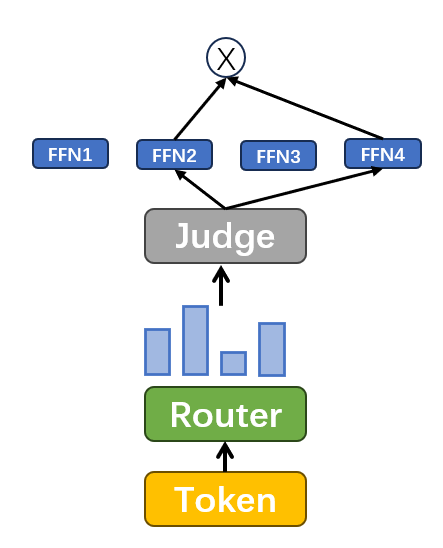
\includegraphics[width=0.3\linewidth]{figures/dynamic gate.png}
    \caption{动态路由的数据分派协议设计}
    \label{fig-dynamic-gate}
    \end{figure}

\subsection{协议设计}
主要设计包含以下步骤:
\begin{enumerate}
    \item 初始阶段:类似于传统的gating策略,系统在计算开始之前需要进行一些初始设置。这包括设定专家容量,确定输入特征,并通过MLP和Softmax层计算权重(如图\ref{fig-dynamic-gate}中的输入Token以及Router计算过程)。这些权重代表每个专家在当前数据上的重要程度或贡献度。
    \item 动态数据分派:与传统的固定分派模式不同,动态路由的数据分派是根据门网络的打分结果进行动态决策。在分派数据时,根据权重得分$f=[f_1, f_2, \cdots, f_E]$从高到低排列,选择得分最高的两个专家,记为$f_{k1}$和$f_{k2}$。如果$f_{k1} - f_{k2}$小于预先设定的阈值Threshold,系统将采用Top-2 Gating的方式将数据发送给这两个专家参与计算。否则,系统按照Top-1 Gating的形式选择得分最高的专家,将数据发送给该专家进行计算。即系统动态地选择使用Top-k(k=1或2)的专家参与计算,根据权重得分的差异性来确定采用哪种分派模式。
    \item 自适应数据发送:在发送数据时,使用All2All Communication的unequal模式,这样可以自适应有效数据长度,从而减少发送不必要的数据(即用于额外padding的0),减少通信量,提高通信效率。
\end{enumerate}

\subsection{系统实现}

对于系统实现而言,采用动态路由的方式确实会带来一些困难,我们在传统的Top-k路由的基础上做出了一些修改以支持动态路由的设计。

\subsubsection{Judge模块实现}
Judge模块接受来自路由器的每个专家(expert)的评分结果,并根据一定的规则进行筛选和判定。该模块的目标是选择最合适的专家进行进一步的决策。

具体而言,Judge模块首先从所有专家的评分结果中选出排名最高的两个专家(即top1和top2),并获取对应的评分分值。然后,它会比较top1和top2的分值差异,判断它们之间是否足够显著。
在比较过程中,Judge模块会使用预先定义的阈值进行判断。如果top1和top2的分值之间的差异小于该阈值,说明它们的评分非常接近,此时将选择top2 gating策略。这意味着在进一步的决策中,会考虑top2专家的意见和贡献。
相反,如果top1和top2的分值之间的差异大于预先定义的阈值,说明它们的评分有较大的差异,此时将选择top1 gating策略。这意味着在进一步的决策中,会主要考虑top1专家的意见和贡献。

通过这样的判定过程,Judge模块能够动态地根据专家评分的差异性选择适当的策略,以最大程度地利用专家的知识和经验,从而对问题进行更准确的决策。


\subsubsection{Unequal All-to-All通信实现}
在传统的 Top-k Gating 中,每个 GPU 在 All-to-All 通信时发送的数据量是均等的,因此在系统实现时比较容易,可以直接调用 PyTorch(NCCL)的 All-to-All 通信实现来完成通信过程。

然而,在采用动态路由后,每个 GPU 上发送的数据量是不均等的。如果仍然按照传统的 Top-2 Gating 的方式发送数据,实际上并未减少通信量。为了解决这个问题,我们采用了 All-to-All 通信的 unequal 模式,该模式不会发送额外的用于填充的0,从而达到减少数据量的目的。

通过实现 unequal 模式的 All-to-All 通信,我们可以根据动态路由的结果,灵活地分派数据并减少通信量。这在系统实现上可能会带来一些挑战,在实现过程中,需要对通信模块进行适当的调整,以支持 unequal 模式的数据传输。

通过在算法上实现动态路由的数据分派模式,在系统上实现unequal All-to-All通信模式。我们可以提高系统的通信效率和计算性能。这样,系统能够根据实际的数据分派需求,灵活地选择数据发送的方式,并减少不必要的通信开销。

\section{本章小结}

MoE模型中的数据分派方式对训练系统的通信量和模型的收敛速度有重要影响。传统的Top-k分派方式在选择专家进行计算时可能会导致不均衡的通信量。为了解决这个问题,我们采用动态路由的数据分派算法设计。该设计通过动态决策,根据门网络的权重得分选择合适的分派方式。具体而言,我们的Gating模块根据权重得分的差异性选择Top-1或Top-2分派方式,从而灵活地分配数据给专家进行计算。在系统实现上,可以采用unequal All-to-All通信模式,减少通信量。通过这样的设计和实现,可以提高系统的通信效率和模型的训练速度。

\endinput